\documentclass{bioinfo}
\copyrightyear{2017} \pubyear{2017}

\access{Advance Access Publication Date: Day Month Year}
\appnotes{Review article}
\graphicspath{{../figures/}}

\newcommand{\comment}[1]{\textcolor{red}{#1}}
\newcommand{\todo}[1]{\colorbox{yellow}{#1}}

\begin{document}
\firstpage{1}

\subtitle{Review}

\title[short Title]{Cardioinformatics: the unmet need to pioneer an emerging field at the nexus of bioinformatics and cardiology}
\author[Sample \textit{et~al}.]{Bohdan B. Khomtchouk\,$^{\text{\sfb 1,}*}$, Diem-Trang Tran\,$^{\text{\sfb 2}}$, Themistocles L. Assimes\,$^{\text{\sfb 3, 4}}$ and Or Gozani\,$^{\text{\sfb 1}}$}
\address{$^{\text{\sf 1}}$Department of Biology, Stanford University, Stanford, CA, USA \\
$^{\text{\sf 2}}$School of Computing, University of Utah, Salt Lake City, UT, USA \\
$^{\text{\sf 3}}$Department of Medicine, Division of Cardiovascular Medicine, Stanford University, Stanford, CA, USA \\
$^{\text{\sf 4}}$VA Palo Alto Health Care System, Palo Alto, CA, USA
}

\corresp{$^\ast$To whom correspondence should be addressed.}

\history{Received on XXXXX; revised on XXXXX; accepted on XXXXX}

\editor{Associate Editor: XXXXXXX}

\abstract{\textbf{Motivation:} Text Text Text Text Text Text Text Text Text Text Text Text Text
Text Text Text Text Text Text Text Text Text Text Text Text Text Text Text Text Text Text Text
Text Text Text Text Text Text Text Text Text Text Text Text Text Text Text Text Text Text Text
Text Text Text Text Text Text
Text Text Text Text Text.\\
\textbf{Results:} Text  Text Text Text Text Text Text Text Text Text  Text Text Text Text Text
Text Text Text Text Text Text Text Text Text Text Text Text Text  Text Text Text Text Text Text\\
\textbf{Availability:} Text  Text Text Text Text Text Text Text Text Text  Text Text Text Text
Text Text Text Text Text Text Text Text Text Text Text Text Text Text  Text\\
\textbf{Contact:} \href{bohdan@stanford.edu}{bohdan@stanford.edu}\\
\textbf{Supplementary information:} Supplementary data are available at \textit{Briefings in Bioinformatics}
online.}

\maketitle

\section{The current status of bioinformatics in cardiovascular disease research}
\begin{figure}
	\centering
	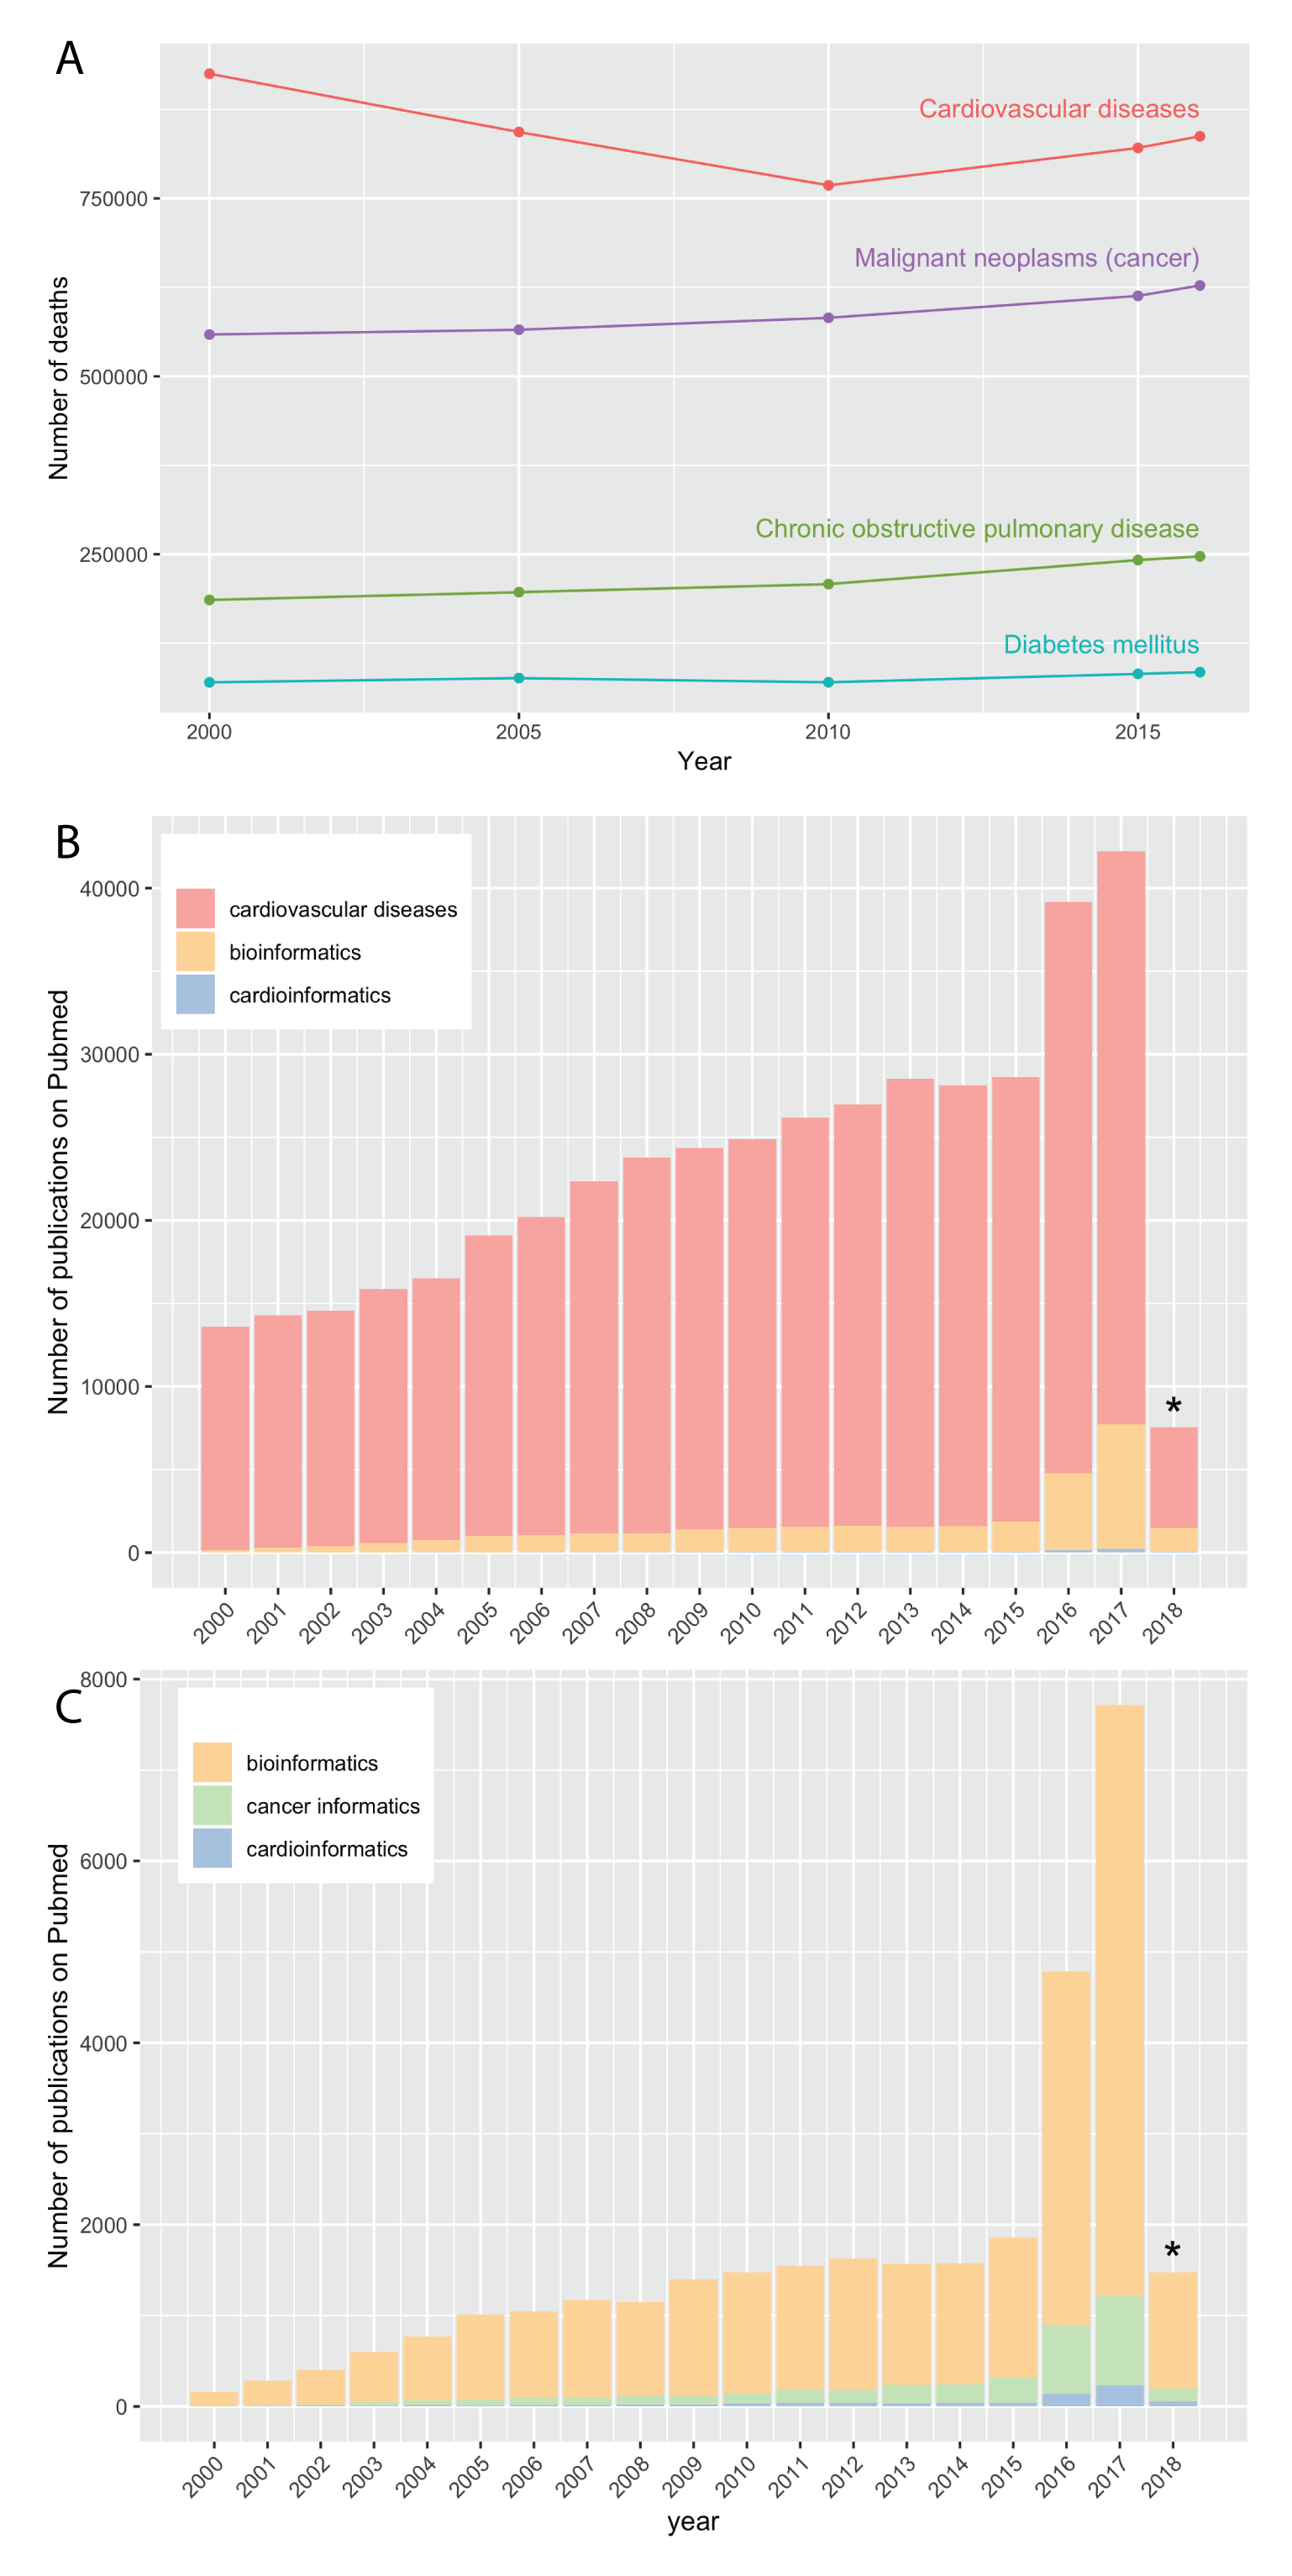
\includegraphics[width=1\linewidth]{figure1}
	\caption{\textbf{A}. Number of deaths by Non-Communicable Diseases in the US. \textbf{B}. \textbf{C}.}
	\label{fig:figure1}
\end{figure}

Medical Subject Heading entry for \textit{cardiovascular diseases}
%{https://www.ncbi.nlm.nih.gov/mesh/68002318} 

\todo{Remove review papers from the count}

\section{The available data}

\begin{figure}[!tpb]%figure1
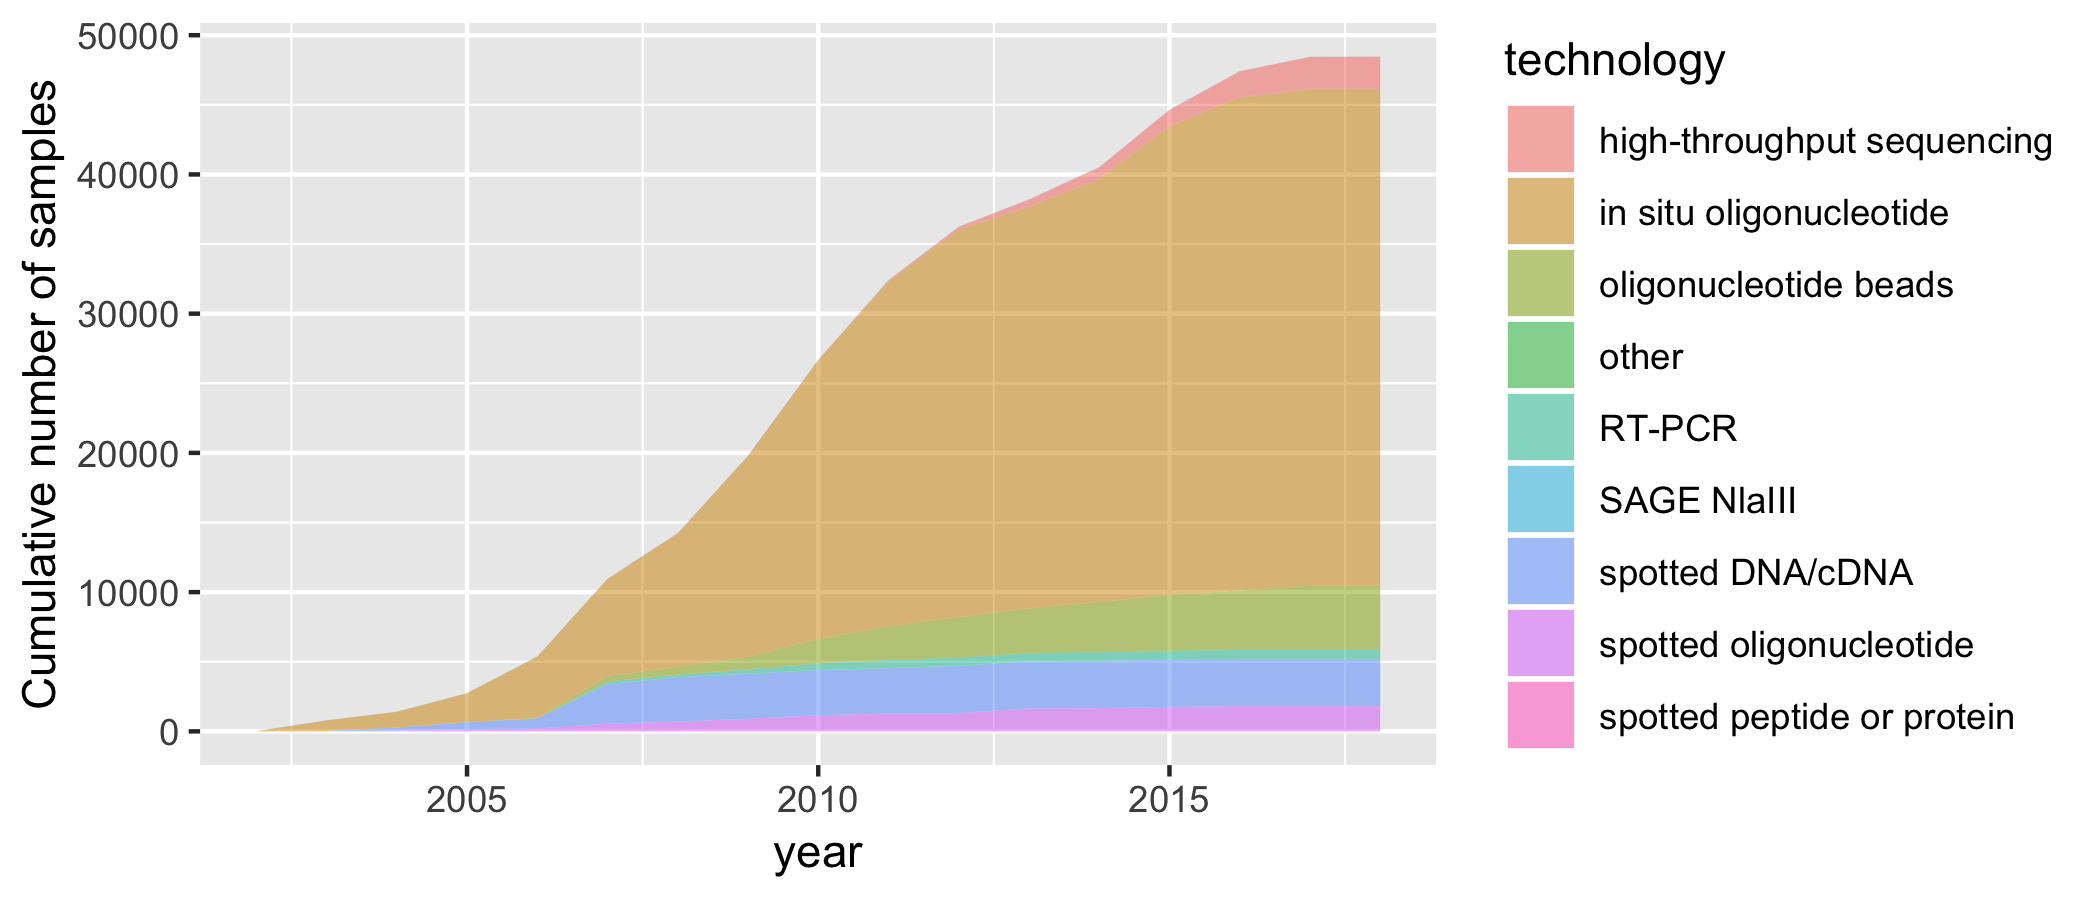
\includegraphics[width=1\linewidth]{gsm_count_by_tech.png}
	\caption{The cumulative number of samples deposited on GEO.}\label{fig:01}
\end{figure}

\section{The possible solutions from bioinformatics}
\subsection{Bioinformatics as a tool-kit}
\subsubsection{Basic research}
for data management, computational analysis, visual representation, etc.

\subsubsection{Clinical application}


\subsection{Bioinformatics as a perspective}


\begin{table}[!t]
	\processtable{Number of samples available on GEO that are of potential use of cardioinformatics research, including those deposited by CVD studies and non-CVD studies.\label{Tab:01}} {\begin{tabular}{@{}llll@{}}\toprule 
    molecule &non-CVD studies & CVD studies \\ \midrule
 genomic DNA &            440 &        8525  \\
   polyA RNA &             89 &         392  \\
   total RNA &           2974 &       39540  \\
       other &             NA &           5  \\
     protein &             NA &           3  \\ \botrule
	\end{tabular}}{This is a footnote}
\end{table}


%\enlargethispage{12pt}




\section*{Acknowledgements}

Text Text Text Text Text Text  Text Text.  \citealp{Boffelli03} might want to know about  text
text text text\vspace*{-12pt}

\section*{Funding}

This work has been supported by the... Text Text  Text Text.\vspace*{-12pt}

%\bibliographystyle{natbib}
%\bibliographystyle{achemnat}
%\bibliographystyle{plainnat}
%\bibliographystyle{abbrv}
\bibliographystyle{bioinformatics}
%
%\bibliographystyle{plain}
%
\bibliography{cardio}



\end{document}
